\newpage
\section{Ôn tập chương 1}
\def\thoigian{90}%--Thời gian
\de{Đề số 1}{Chương I. Hàm số lượng giác và phương trình lượng giác}


\begin{center}
	\textbf{PHẦN 1 - CÂU TRẮC NGHIỆM BỐN PHƯƠNG ÁN}
\end{center}
\Opensolutionfile{ans}[ans/ans-TN-1D1-DE1]
%%%=============EX_1=============%%%
\begin{ex}%[1D1N1-2]%[Dự án D - đợt 2 NH24-25- Hứa Chí Ninh]
	Góc có số đo $\dfrac{\pi}{12}$ đổi sang độ là
	\choice
	{\True  $15^\circ$}
	{$16^\circ$}
	{$17^\circ 30'$}
	{$14^\circ$}
	\loigiai{
		Ta có $\dfrac{\pi}{12}\,\mathrm{rad}=\left(\dfrac{\pi}{12}\cdot \dfrac{180}{\pi}\right)^\circ = 15^\circ$.
	}
\end{ex}

%%%=============EX_2=============%%%
\begin{ex}%[1D1H1-3]%[Dự án D - đợt 2 NH24-25- Hứa Chí Ninh]
	\immini{Góc lượng giác trên hình có số đo bao nhiêu?
		\choice
		{$\dfrac{\pi}{2}$}
		{\True $\dfrac{13\pi}{2}$}
		{$-\dfrac{13\pi}{2}$}
		{$\dfrac{5\pi}{2}$}}
	{	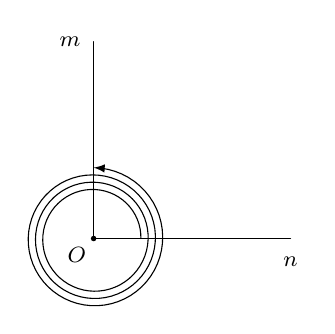
\begin{tikzpicture}[>=stealth,line join=round,line cap=round,font=\footnotesize,scale=1]
			\def\r{2.5}
			\path 
			(0,0) coordinate (O)
			(\r,0) coordinate (n)
			(90:\r) coordinate (m)
			;
			\draw (n)--(O)--(m);
			\draw[->,domain=0:1170,variable=\t,samples=200,>=latex]
			plot ({0.6*(\t+2*1170)*cos(\t)/(2*1170)},
			{0.6*(\t+ 2*1170)*sin(\t)/(2*1170)})
			;
			\fill[black] (O) circle (1pt);
			\foreach \l/\g in {n/-90,m/180,O/-135}
			\draw[fill=black] (\l) +(\g:.3) node{$\l$};
	\end{tikzpicture}}
	\loigiai{
		Dựa vào hình vẽ, ta thấy góc lượng giác đã cho có số đo $\dfrac{\pi}{2}+3\cdot 2\pi= \dfrac{13\pi}{2}$.
	}
\end{ex}

%%%=============EX_3=============%%%
\begin{ex}%[1D1N3-1]%[Dự án D - đợt 2 NH24-25- Hứa Chí Ninh]
	Với mọi $a,b$, ta có $\sin(a-b)$ bằng
	\choice
	{$\sin a \sin b-\cos a\cos b$}
	{$\sin b \cos a- \sin a\cos b$}
	{\True $\sin a \cos b - \cos a \sin b$}
	{$\sin a \cos b + \cos a\sin b$}
	\loigiai{Theo công thức cộng, ta có $\sin (a-b) = \sin a \cos b -\cos a \sin b$.	
	}
\end{ex}

%%%=============EX_4=============%%%
\begin{ex}%[1D1H3-2]%[Dự án D - đợt 2 NH24-25- Hứa Chí Ninh]
	Cho $a,b \in \left[0;\dfrac{\pi}{2}\right]$ thỏa mãn $\sin a = \cos b = \dfrac{3}{5}$. Khi đó $\sin (a+b)$ bằng
	\choice
	{$\dfrac{24}{25}$}
	{\True $1$}
	{$0$}
	{$-\dfrac{7}{25}$}
	\loigiai{Ta có $a,b \in \left[0;\dfrac{\pi}{2}\right]$, suy ra $\cos a>0$ và $\sin b >0$.\\
		Lại có $\sin^2a + \cos^2a=\sin^2b+\cos^2b=1$, suy ra $\cos a= \sqrt{1-\left(\dfrac{3}{5}\right)^2}=\dfrac{4}{5}$ và $\sin b = \sqrt{1-\left(\dfrac{3}{5}\right)^2}=\dfrac{4}{5}$.\\
		Suy ra $\sin (a+b) = \sin a \cos b + \cos a \sin b = \dfrac{3}{5}\cdot\dfrac{3}{5} + \dfrac{4}{5}\cdot\dfrac{4}{5} = 1$. 
		
	}
\end{ex}

%%%=============EX_5=============%%%
\begin{ex}%[1D1N3-1]%[Dự án D - đợt 2 NH24-25- Hứa Chí Ninh]
	Thu gọn $\sin a \sin b - \cos a \cos b$, ta được
	\choice
	{\True $-\cos (a+b)$}
	{$\cos (a-b)$}
	{$\cos (a+b)$}
	{$-\cos (a-b)$}
	\loigiai{
		Ta có $\sin a \sin b - \cos a\cos b = -(\cos a\cos b - \sin a \sin b) = -\cos (a+b)$.
	}
\end{ex}

%%%=============EX_6=============%%%
\begin{ex}%[1D1N3-2]%[Dự án D - đợt 2 NH24-25- Hứa Chí Ninh]
	Cho $a$, $b$ thỏa mãn $\tan a = \tan b = 2$. Tính $\tan (a+b)$.
	\choice
	{\True $-\dfrac{4}{3}$}
	{$\dfrac{4}{3}$}
	{$0$}
	{$\dfrac{3}{4}$}
	\loigiai{Áp dụng công thức cộng, ta có $\tan (a+b) = \dfrac{\tan a + \tan b}{1 - \tan a \tan b} = \dfrac{2+2}{1-2\cdot2} = -\dfrac{4}{3}$.}
\end{ex}
%Câu 7

%%%=============EX_7=============%%%
\begin{ex}%[1D1H3-2]%[Dự án D - đợt 2 NH24-25- Hứa Chí Ninh]
	Biểu thức nào sau đây bằng $\cos\left(x-\dfrac{\pi}{3}\right)$?
	\choice
	{$\dfrac{1}{2} \cos x - \dfrac{\sqrt{3}}{2}\sin x$}
	{$\dfrac{\sqrt{3}}{2}\cos x - \dfrac{1}{2}\sin x$}
	{\True $\dfrac{1}{2} \cos x + \dfrac{\sqrt{3}}{2}\sin x$}
	{$\dfrac{\sqrt{3}}{2}\cos x + \dfrac{1}{2}\sin x$}
	\loigiai{
		Áp dụng công thức cộng, ta có $\cos \left(x-\dfrac{\pi}{3}\right) = \cos x \cos \dfrac{\pi}{3} + \sin x \sin \dfrac{\pi}{3} = \dfrac{1}{2}\cos x + \dfrac{\sqrt{3}}{2}\sin x$.
	}
\end{ex}

%%%=============EX_8=============%%%
\begin{ex}%[1D1N4-2]%[Dự án D - đợt 2 NH24-25- Hứa Chí Ninh]
	Tập xác định của hàm số $y=\sqrt{1-\cos 2x}$ là
	\choice
	{\True $\mathscr{D}=\mathbb{R}$}
	{$\mathscr{D}=[0;1]$}
	{$\mathscr{D}=[-1;1]$}
	{$\mathscr{D}=\mathbb{R}\setminus\left\{k\pi, k\in\mathbb{Z}\right\}$}
	\loigiai{
		Ta có  $-1\leq\cos 2x\leq 1\Rightarrow 1-\cos 2x\geq 0, \,\forall x\in\mathbb{R}$.\\
		Vậy tập xác định của hàm số là $\mathscr{D}=\mathbb{R}$.}
\end{ex}

%%%=============EX_9=============%%%
\begin{ex}%[1D1H4-6]%[Dự án D - đợt 2 NH24-25- Hứa Chí Ninh]
	Giá trị lớn nhất $M$ và giá trị nhỏ nhất $m$ của hàm số $y=\dfrac{1+4\cos^2x}{3}$ lần lượt là
	\choice{$M=3$ và $m=2$}
	{\True $M=\dfrac{5}{3}$ và $m=\dfrac{1}{3}$}
	{$M=\dfrac{5}{3}$ và $m=-1$}
	{$M=3$ và $m=-\dfrac{2}{3}$}
	\loigiai{
		Vì $0\leq\cos^2x\leq1$ nên $\dfrac{1}{3}\leq\dfrac{1+4\cos^2x}{3}\leq\dfrac{5}{3}$\\
		Vậy $\min y=\dfrac{1}{3}$, đạt được khi $\cos x=0\Leftrightarrow x=\dfrac{\pi}{2}+k\pi$, $k\in\mathbb{Z}$.\\
		$\max y=\dfrac{5}{3}$, đạt được khi $\cos^2 x=1\Leftrightarrow \cos x=\pm 1\Leftrightarrow x=k\pi$, $k\in\mathbb{Z}$.
	}
\end{ex}

%%%=============EX_10=============%%%
\begin{ex}%[1D1N4-1]%[Dự án D - đợt 2 NH24-25- Hứa Chí Ninh]
	Hàm số $y=\tan x$ tuần hoàn với chu kì là bao nhiêu?
	\choice
	{\True $T=\pi$}
	{$T=2\pi$}
	{$T=\dfrac{\pi}{2}$}
	{$T=\dfrac{\pi}{4}$}
	\loigiai{
		Hàm số $y=\tan x$ tuần hoàn với chu kì $\pi$.
	}
\end{ex}

%%%=============EX_11=============%%%
\begin{ex}%[1D1N5-3]%[Dự án D - đợt 2 NH24-25- Hứa Chí Ninh]
	Phương trình $\sin x=\dfrac{\sqrt{3}}{2}$ có tập nghiệm là
	\choice
	{$S=\left\{\dfrac{\pi}{6}+k2\pi;\dfrac{5\pi}{6}+k2\pi,k\in \mathbb{Z}\right\}$}
	{$S=\left\{\dfrac{\pi}{3}+k2\pi;-\dfrac{\pi}{3}+k2\pi,k\in \mathbb{Z}\right\}$}
	{\True $S=\left\{\dfrac{\pi}{3}+k2\pi;\dfrac{2\pi}{3}+k2\pi,k\in \mathbb{Z}\right\}$}
	{$S=\left\{\dfrac{\pi}{3}+k2\pi;-\dfrac{2\pi}{3}+k2\pi,k\in \mathbb{Z}\right\}$}
	\loigiai{
		Ta có $\sin x=\dfrac{\sqrt{3}}{2}\Leftrightarrow \sin x=\sin \dfrac{\pi}{3}\Leftrightarrow \hoac{&x=\dfrac{\pi}{3}+k2\pi \\&x=\dfrac{2\pi}{3}+k2\pi}\, (k\in \mathbb{Z})$.}
\end{ex}

%%%=============EX_12=============%%%
\begin{ex}%[1D1H5-3]%[Dự án D - đợt 2 NH24-25- Hứa Chí Ninh]
	Tập nghiệm của phương trình $\cos 2x=\dfrac{\sqrt{3}}{2}$ là
	\choice
	{\True $x=\pm \dfrac{\pi}{12}+k\pi,\, k\in \mathbb{Z} $}
	{$x=\pm \dfrac{\pi}{6}+k\pi,\, k\in \mathbb{Z} $}
	{$x=-\dfrac{\pi}{12}+k\pi, \, k\in \mathbb{Z}$}
	{$x=\dfrac{\pi}{12}+k\pi, \, k\in \mathbb{Z}$}
	\loigiai{
		Ta có $\cos 2x=\dfrac{\sqrt{3}}{2}\Leftrightarrow 2x=\pm \dfrac{\pi}{6}+k2\pi \Leftrightarrow x=\pm \dfrac{\pi}{12}+k\pi ,\,k\in \mathbb{Z}$.}
\end{ex}

\Closesolutionfile{ans}
%\begin{center}
%	\textbf{ĐÁP ÁN}
%	\inputansbox{10}{ans/ans-TN-1D1-DE1}	
%\end{center}

\begin{center}
	\textbf{PHẦN 2 - CÂU TRẮC NGHIỆM ĐÚNG SAI}
\end{center}

\Opensolutionfile{ans}[ans/ans-DS-1D1-DE1]
\setcounter{ex}{0}
%%%=============EX_1=============%%%
\begin{ex}%[1D1H2-2]%[Dự án D - đợt 2 NH24-25- Hứa Chí Ninh]
	\immini{Cho đường tròn lượng giác gốc $A$, gọi $M\left(x_0 ; y_0\right)$ là điểm biểu diễn góc lượng giác có số đo $\alpha$ (tham khảo hình vẽ).
		\choiceTF
		{ $\sin \alpha=x_0$}
		{ $\cos \alpha=y_0$}
		{ $\tan \alpha=\dfrac{x_0}{y_0}$}
		{ \True  $\cot \alpha>0$}
		\loigiai
		{		Ta có
			\begin{itemchoice}
				\itemch $\sin \alpha=y_0$.
				\itemch $\cos \alpha=x_0$.
				\itemch $\tan \alpha=\dfrac{y_0}{x_0}$.
				\itemch Vì $x_0>0 ; y_0>0$ nên $\cot \alpha=\dfrac{x_0}{y_0}>0$.
			\end{itemchoice}
		}
	}{
		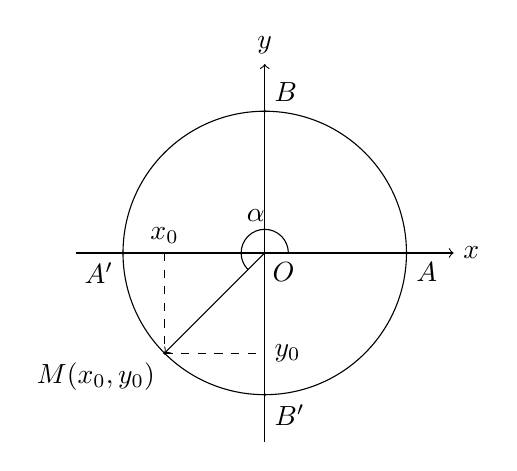
\begin{tikzpicture}[scale=0.6]
			% Vẽ đường tròn bán kính 3
			\draw[black] (0,0) circle(3);
			% Ox, Oy
			\draw[->] (-4,0) -- (4,0) node[right] {$x$};
			\draw[->] (0,-4) -- (0,4) node[above] {$y$};
			% Các điểm A, A', B, B'
			\fill (3,0) circle(1pt) node[below right] {$A$};
			\fill (-3,0) circle(1pt) node[below left]  {$A'$};
			\fill (0,3) circle(1pt) node[above right] {$B$};
			\fill (0,-3) circle(1pt) node[below right] {$B'$};
			% Điểm M( x0, y0 ) trên đường tròn (ví dụ x0=-2.12,y0=-2.12)
			\coordinate (M) at (-2.12,-2.12);
			\fill (M) circle(1pt) node[below left] {$M(x_0,y_0)$};
			% Dựng hình chiếu
			\draw[dashed] (M|-0,0) node[above] {$x_0$} -- (M);
			\draw[dashed] (M) -- (0,0|-M);
			\node [right] at (0,-2.12) {$y_0$};
			% Vẽ OM và góc alpha
			\draw[black,->] (0,0) -- (M);
			\draw[black] (0.5,0) arc(0:{225}:0.5) node[midway, above] {$\alpha$};
			% Gốc O
			\node at (0.4,-0.4) {$O$};
	\end{tikzpicture}}
\end{ex}

\begin{ex}%[1D1V4-6]
	Cho hàm số $f(x)=\dfrac{5\sin x+3}{\cos x}$.
	\choiceTF
	{$y(\pi)=3$}
	{\True Tập xác định của hàm số là $\mathscr{D}=\mathbb{R}\setminus \left\{ \dfrac{\pi }{2}+k\pi,\,k\in \mathbb{Z} \right\}$}
	{Hàm số tuần hoàn với chu kỳ $\pi$}
	{Đồ thị hàm số cắt trục hoành tại $2$ điểm trong $[0;\pi]$}
	\loigiai{
		\begin{itemchoice}
			\itemch $y(\pi)=\dfrac{5\sin \pi+3}{\cos \pi}=\dfrac{3}{-1}=-3$.
			\itemch Hàm số $y=\dfrac{5\sin x+3}{\cos x}$ xác định khi $\cos x \ne 0 \Leftrightarrow x \ne \dfrac{\pi}{2} + k\pi$, $k \in \mathbb{Z}$.\\
			Vậy tập xác định của hàm số là $\mathscr{D}=\mathbb{R}\setminus \left\{ \dfrac{\pi }{2}+k\pi,\,k\in \mathbb{Z} \right\}$.
			\itemch Ta có $f(0+\pi)=f(\pi)=-3$.\\
			$f(0)=3$.\\
			Vì $f(0+\pi)\ne f(0)$ nên hàm số không tuần hoàn với chu kỳ $\pi$.
			\itemch Phương trình hoành độ giao điểm của $y=f(x)$ và trục hoành là $\dfrac{5\sin x+3}{\cos x}=0
			\Rightarrow 5\sin x+3=0
			\Rightarrow \sin x=-\dfrac{3}{5}$. \hfill(1)\\
			Trên $[0;\pi]$, $\sin x\ge 0$ nên $(1)$ vô nghiệm.\\
			Do đó đồ thị hàm số và trục hoành không có điểm chung trên $[0;\pi]$.
		\end{itemchoice}
		
	}
\end{ex}
 
\Closesolutionfile{ans}
%\inputansbox[2]{2}{ans/ans-DS-1D1-DE1}

\begin{center}
	\textbf{PHẦN 3 - CÂU TRẮC NGHIỆM TRẢ LỜI NGẮN}
\end{center}
\setcounter{ex}{0}
\Opensolutionfile{ans}[ans-KQ-1D1-DE1]
%%%=============EX_1=============%%%
\begin{ex}%[1D1H2-2]%[Dự án D - đợt 2 NH24-25- Hứa Chí Ninh]
	Cho $x \in [0;\pi]$ thỏa mãn $\cos x = \dfrac{3}{5}$. Tính $\tan \left(x + \dfrac{\pi}{4}\right)$.
	\shortans{$-7$}
	\loigiai{
		Ta có $\cos^2x+\sin^2x = 1$, suy ra $\sin^2x = 1-\cos^2x = 1-\left(\dfrac{3}{5}\right)^2 = \dfrac{16}{25}$.\\
		Vì $x\in [0;\pi]$ nên $\sin x \ge 0$, suy ra $\sin x = \sqrt{\dfrac{16}{25}} = \dfrac{4}{5}$.\\
		Ta có $\tan x = \dfrac{\sin x}{\cos x} = \dfrac{4}{5}:\dfrac{3}{5} = \dfrac{4}{3}$, suy ra $\tan \left(x+\dfrac{\pi}{4}\right) = \dfrac{\tan x + \tan \dfrac{\pi}{4}}{1 - \tan x\tan \dfrac{\pi}{4}} = \dfrac{1+\dfrac{4}{3}}{1-\dfrac{4}{3}} = -7$.
	}
\end{ex}

%%%=============EX_2=============%%%
\begin{ex}%[1D1H4-6]%[Dự án D - đợt 2 NH24-25- Hứa Chí Ninh]
	Tìm giá trị lớn nhất của hàm số $y=3-\sin 2 x$ trên đoạn $\left[ 0; \dfrac{\pi}{2}\right]$.
	\shortans{$3$}
	\loigiai
	{\immini
		{Ta có $x\in \left[ 0; \dfrac{\pi}{2}\right]\Rightarrow 2x\in \left[ 0; \pi\right]$.\\
			Với mọi $2x\in \left[ 0; \pi\right]$ ta có
			\allowdisplaybreaks
			\begin{eqnarray*}
				& & 0\leq \sin 2x\leq 1\\
				&\Leftrightarrow& -1\leq -\sin 2x\leq 0\\
				&\Leftrightarrow&2\leq 3-\sin 2x\leq 3.
			\end{eqnarray*}
			Vậy $M=\max\limits_{x \in \left[ 0; \tfrac{\pi}{2}\right]} y=3$ khi $x=0$.
		}
		{
			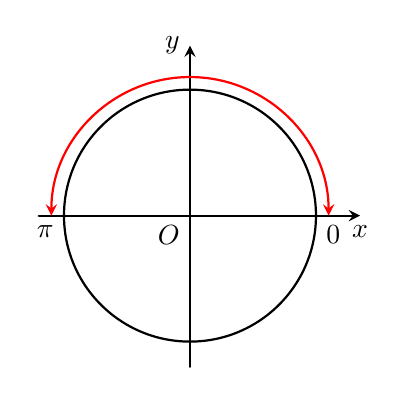
\begin{tikzpicture}[line join=round, line cap=round,>=stealth,thick,scale=0.8]
				\tikzset{label style/.style={font=\footnotesize}}
				\draw[->] (-2.4,0)--(2.7,0) node[below] {$x$};
				\draw[->] (0,-2.4)--(0,2.7) node[left] {$y$};
				\draw (0,0) node [below left] {$O$};
				\draw (2,0) node [below right] {$0$};
				\draw (-2,0) node [below left] {$\pi$};
				\draw (0,0) circle (2);
				\draw[red,<->] (2.2,0) arc (0:180:2.2 cm);
			\end{tikzpicture}
		}	
	}
\end{ex}

%%%=============EX_3=============%%%
\begin{ex}%[1D1H5-3]%[Dự án D - đợt 2 NH24-25- Hứa Chí Ninh]
	Phương trình $\tan 5x-\tan x=0$ có bao nhiêu nghiệm thuộc nửa khoảng $\left[0;\pi\right)$?
	\shortans{$3$}
	\loigiai{
		Điều kiện $\heva{&5x\ne \dfrac{\pi}{2}+k\pi \\&x\ne \dfrac{\pi}{2}+k\pi}\Leftrightarrow \heva{&x\ne \dfrac{\pi}{10}+k\dfrac{\pi}{2} \\&x\ne \dfrac{\pi}{2}+k\pi},k\in \mathbb{Z}$.\\
		Ta có $\tan 5x-\tan x=0 \Leftrightarrow \tan 5x=\tan x$
		$\Leftrightarrow 5x=x+k\pi $
		$\Leftrightarrow x=\dfrac{k\pi}{4}$ ($k\in \mathbb{Z}$).\\
		Do $x\in \left[0;\pi\right)$ và kết hợp với điều kiện suy ra $x\in \left\{0;\dfrac{\pi}{4};\dfrac{3\pi}{4}\right\}$.\\
		Vậy phương trình $\tan 5x-\tan x=0$ có $3$ nghiệm thuộc nửa khoảng $\left[0;\pi\right)$.}
\end{ex}
\begin{ex}%[1D1V5-6]
	Một cây cầu có dạng cung $AB$ của đồ thị hàm số $y=4{,}8 \cdot \cos \dfrac{x}{9}$ và được mô tả trong hệ trục toạ độ với đơn vị trục là mét như ở hình vẽ. Một sà lan chở khối hàng hoá được xếp thành hình hộp chữ nhật với độ cao $3{,}6$ m so với mực nước sông. Hỏi chiều rộng của khối hàng hóa đó lớn nhất là bao nhiêu mét để sà lan có thể đi qua được gầm cầu (làm tròn kết quả đến hàng đơn vị)?
	\shortans[]{$13$}
	\begin{center}
		\begin{tikzpicture}[>=stealth,scale=0.3]
			\draw[->] (-17,0) -- (17,0)node[above]{$x$};
			\draw[->] (0,-2) -- (0,6) node[left] {$y$};
			\draw (0,0)node[below left]{$O$};
			\clip (-15,-3)rectangle(15,5);
			\draw[samples=150,smooth,domain=-14.137:14.137] plot(\x,{4.8*cos(\x/9 r)});
			\node at (-14.14,0)[below]{$-\dfrac{9\pi}{2}$};
			\node at (-14.14,0)[above]{$A$};
			\node at (14.14,0)[below]{$\dfrac{9\pi}{2}$};
			\node at (14.14,0)[above]{$B$};
		\end{tikzpicture}
	\end{center}
	\loigiai{
		Với mỗi điểm $M(x;y)$ nằm trên mặt cây cầu, khoảng cách từ điểm $M$ đến mặt nước tương ứng với giá trị tung độ $y$ của $M$. Xét phương trình 
		$$4{,}8\cos \dfrac{x}{9}=3{,}6\Leftrightarrow \cos \dfrac{x}{9}=\dfrac{3}{4}.$$
		Do $x\in \left[-\dfrac{9\pi}{2};\dfrac{9\pi}{2}\right]$ nên $\dfrac{x}{9}\in \left[-\dfrac{\pi}{2};\dfrac{\pi}{2}\right]$. \\
		Từ phương trình $\cos \dfrac{x}{9}=\dfrac{3}{4}$ với $\dfrac{x}{9}\in \left[-\dfrac{\pi}{2};\dfrac{\pi}{2}\right]$, ta có $\dfrac{x}{9}\approx \pm 0{,}7227$. Khi đó $2|x|\approx 13$.\\
		Vậy chiều rộng của khối hàng lớn nhất là $13$ mét để có thể đi qua được gầm cầu.
	}
\end{ex}
\Closesolutionfile{ans}

\begin{center}
	\textbf{PHẦN 4 - TỰ LUẬN}
\end{center}
\setcounter{ex}{0}
%%%=============EX_1=============%%%
\begin{ex}%[1D1H2-1]%[Dự án D - đợt 2 NH24-25- Hứa Chí Ninh]
	Tính $\tan \left(x+\dfrac{\pi}{4}\right)$ biết $\cos x = \dfrac{2}{3}$ và $0<x<\pi$.
	\loigiai{
		Ta có $\sin^2 x + \cos^2 x = 1 \Rightarrow \sin^2x = 1-\cos^2x = 1-\left(\dfrac{2}{3}\right)^2 = \dfrac{5}{9}$.\\
		Vì $0<x<\pi$ nên $\sin x >0$, suy ra $\sin x = \sqrt{\dfrac{5}{9}} = \dfrac{\sqrt{5}}{3}$.\\
		Do đó $\tan x = \dfrac{\sin x}{\cos x} = \dfrac{\sqrt{5}}{3}:\dfrac{2}{3} = \dfrac{\sqrt{5}}{2}$.\\
		Suy ra $\tan \left(x + \dfrac{\pi}{4}\right) = \dfrac{\tan x + \tan \dfrac{\pi}{4}}{1-\tan x\tan \dfrac{\pi}{4}} = \dfrac{\dfrac{\sqrt{5}}{2}+1}{1-\dfrac{\sqrt{5}}{2}\cdot1} = \dfrac{\sqrt{5}+2}{2-\sqrt{5}} = \dfrac{\left(\sqrt{5}+2\right)^2}{2^2-\sqrt{5}^2} = -9-4\sqrt{5}$.\\
		Vậy $\tan \left(x+\dfrac{\pi}{4}\right) = -9-4\sqrt{5}$.
	}
\end{ex}

%%%=============EX_2=============%%%
\begin{ex}%[1D1V4-6]
	Tìm giá trị lớn nhất, giá trị nhỏ nhất của hàm số $f(x)=-2\sin^{2}x+\sin{x}+2$.
	\loigiai{
		Đặt $t=\sin{x}$ với $t\in [-1;1]$, ta có
		$f(t)=-2t^2+t+2$ với $t\in [-1;1]$.\\
		Bảng biến thiên
		\begin{center}
			
\begin{tikzpicture}
				\tkzTabInit[nocadre=false,lgt=1,espcl=3.5,deltacl=0.6]
				{$t$ /0.7,$f(t)$ /2.3}
				{$-1$,$\tfrac{1}{4}$,$1$}
				\tkzTabVar{ -/$-1$,+/$\dfrac{17}{8}$,-/$1$}
			\end{tikzpicture}
		\end{center}
		Từ bảng biến thiên trên suy ra $\max\limits_{t\in [-1;1]} f(t)=\max\limits_{x\in \mathbb{R}} f(x)=\dfrac{17}{8}$; $\min\limits_{t\in [-1;1]} f(t)=\min\limits_{x\in \mathbb{R}} f(x)=-1$.
	}
\end{ex}

%%%=============EX_3=============%%%
\begin{ex}%[1D1H5-5]%[Dự án D - đợt 2 NH24-25- Hứa Chí Ninh]
	Giải phương trình $3\cot^2\left(5x+40^\circ\right)=1$.
	\loigiai{
		Ta có $3\cot^2\left(5x+40^\circ\right)=1\Leftrightarrow\cot\left(5x+40^\circ\right)=\pm\dfrac{\sqrt{3}}{3}$.
		\begin{itemize}
			\item $\cot\left(5x+40^\circ\right)=\dfrac{\sqrt{3}}{3}=\cot 60^\circ\Leftrightarrow 5x+40^\circ=60^\circ+k180^\circ\Leftrightarrow x=4^\circ+k360^\circ, k\in\mathbb{Z}$.
			\item $\cot\left(5x+40^\circ\right)=-\dfrac{\sqrt{3}}{3}=\cot \left(-60^\circ\right)\Leftrightarrow 5x+40^\circ=-60^\circ+k180^\circ\Leftrightarrow x=-20^\circ+k360^\circ, k\in\mathbb{Z}$.
		\end{itemize}
	}
\end{ex}
\begin{ex}%[1D1V6-6]
	Giải phương trình $1+\cot 2x=\dfrac{2(1-\cos2x)}{\sin^22x}$.
	\loigiai{
		Điều kiện $\sin2x\neq 0\Leftrightarrow 2x\neq k\pi \Leftrightarrow x\neq k\dfrac{\pi}{2},\, k\in \mathbb{Z}$.\\
		Ta có 
		\allowdisplaybreaks
		\begin{eqnarray*}
			&&1+\cot 2x=\dfrac{2(1-\cos2x)}{\sin^22x}\\
			&\Leftrightarrow& \sin^2 2x+\sin 2x\cos 2x=1-\cos 2x\\ &\Leftrightarrow& (\sin2x+1)(\sin2x+\cos2x-2)=0\\ &\Leftrightarrow& \hoac{&\sin2x=-1\\&\sin2x+\cos2x=2.}
		\end{eqnarray*}
		Vì $\sin2x+\cos2x=\sqrt{2}\sin\left(2x+\dfrac{\pi}{4}\right)$ nên phương trình $\sin2x+\cos2x=2 \Leftrightarrow \sin\left(2x+\dfrac{\pi}{4}\right)=\sqrt{2}$, do đó phương trình này vô nghiệm.\\
		Phương trình $\sin2x=-1$ có nghiệm $x=-\dfrac{\pi}{4}+k\dfrac{\pi}{2}$, $k\in\mathbb{Z}$.
	}
\end{ex}